% Created 2018-06-25 Mo 13:07
% Intended LaTeX compiler: pdflatex
\documentclass[11pt]{scrartcl}
\usepackage[utf8]{inputenc}
\usepackage[T1]{fontenc}
\usepackage{graphicx}
\usepackage{grffile}
\usepackage{longtable}
\usepackage{wrapfig}
\usepackage{rotating}
\usepackage[normalem]{ulem}
\usepackage{amsmath}
\usepackage{textcomp}
\usepackage{units}
\usepackage{amssymb}
\usepackage{capt-of}
\usepackage{hyperref}
\usepackage{capt-of}
\usepackage[framemethod=TikZ]{mdframed}
\usepackage[authoryear,round]{natbib}
\author{}
\date{}
\title{Response to reviewer 2}
\hypersetup{
 pdfauthor={Simon Pfreundschuh},
 pdftitle={},
 pdfkeywords={},
 pdfsubject={},
 pdfcreator={Emacs 24.5.1}, 
 pdflang={English}}

\RequirePackage[normalem]{ulem} %DIF PREAMBLE
\RequirePackage{luacolor}\definecolor{RED}{rgb}{1,0,0}\definecolor{BLUE}{rgb}{0,0,1} %DIF PREAMBLE
\providecommand{\DIFadd}[1]{{\protect\textcolor{blue}{\uwave{#1}}}} %DIF PREAMBLE
\providecommand{\DIFdel}[1]{{\protect\textcolor{red}{\sout{#1}}}}                      %DIF PREAMBLE
%DIF SAFE PREAMBLE %DIF PREAMBLE
\providecommand{\DIFaddbegin}{} %DIF PREAMBLE
\providecommand{\DIFaddend}{} %DIF PREAMBLE
\providecommand{\DIFdelbegin}{} %DIF PREAMBLE
\providecommand{\DIFdelend}{} %DIF PREAMBLE
%DIF FLOATSAFE PREAMBLE %DIF PREAMBLE
\providecommand{\DIFaddFL}[1]{\DIFadd{#1}} %DIF PREAMBLE
\providecommand{\DIFdelFL}[1]{\DIFdel{#1}} %DIF PREAMBLE
\providecommand{\DIFaddbeginFL}{} %DIF PREAMBLE
\providecommand{\DIFaddendFL}{} %DIF PREAMBLE
\providecommand{\DIFdelbeginFL}{} %DIF PREAMBLE
\providecommand{\DIFdelendFL}{} %DIF PREAMBLE

\newenvironment{change}[1][]{%
  \begin{mdframed}[frametitle={Line #1:}]%
}{%
  \end{mdframed}%
}

\begin{document}

\maketitle

\setlength{\parindent}{0cm}

We thank the referee for the time he/she has put on reading our manuscript and providing
feedback.

Based on the combined comments of the referees, we have decided to implement these general
changes:

\begin{itemize}
\item We will switch to an airborne measurement set-up
\item The test in the result section will be significantly shorter
\item Redundant results for scene 2 will be placed in an appendix
\item The selection of tested retrieval habits will be revised/changed
\end{itemize}

Below we respond to the main questions raised by the referee, and outline how we will
revise the manuscript.


\section{Major points}

\subsection*{Review comment 1}

A major aspect of the study concerns the representation of the particle size
distribution which is retrieved by two free parameters (different from the 2
moments of the atmospheric model GEM used to provide the test scenes) and the
assumptions of the particle type. The difficulty of connecting atmospheric model
output to single scattering properties (which is one of the fundamental
assumptions) could be better explained. The motivation why the authors choose
their approach and why they test certain settings need to be discussed in the
beginning. Couldn’t Tab. 1 and 4 be combined and better explained which is used
for which purpose? Why is cloud ice the same and GEMsnow and GEMGraupel different
in both?

\subsubsection*{Author response:}

We agree with the comment that the rather arbitrary choice of tested particles
is a weak spot of the study. To improve this, the experiments will be repeated
with a more principled selection of particles. The new selection is based on the
particle properties described in \citet{ekelund19} and covers a broader range of
mass-size relationships and scattering parameters. In particular, the GemSnow
model has been removed from the selection of test particles because it does not
cover small ice particle sizes.

We propose to make the following changes to the manuscript:

\begin{itemize}
\item Add a paragraph to the description of the GEM test scenes which explains
  the particle models that have been developed to match the assumptions of
  the GEM microphysics scheme and that are used to simulate observations.
\item Add a paragraph to the description of the retrieval implementation that
  explains the difficulties of representing the complex mixture of different
  particle with a single particle model and that we therefore test several
  of them.
\item To combined Tab. 1 and 4. into a single table.
\end{itemize}

%The following changes will be introduced in the manuscript:
%
%\begin{itemize}
%\item To explain how hydrometeor concentration from the model scenes are
%  connected to ice particle models  the following paragraph will be added
%  to sections describing the GEM model scenes:
%
%  \begin{change}[101]
%\DIFaddbegin \DIFadd{In order to simulate microwave observations for the GEM model scenes, the
%hydrometeor classes in the model must be associated with particle models that
%define their shape and thus their radiometric properties. The ARTS
%single-scattering database contains particle models that were designed to be
%consistent with the six classes of hydrometeors of GEM microphysics scheme. Rain
%and liquid cloud drops are modeled as liquid spheres. Ice, snow, hail and
%graupel are represented using the GemCloudIce, GemSnow, GemHail and GemGraupel
%particle models. The properties of the particle models used for the frozen
%hydrometeor types are listed together with their parameters in
%Tab.~3.}
%\DIFaddend
%  \end{change}
%
%\item To describe the difficulties of representing the complex mixture of
%  particle shapes from the GEM model scenes in the retrieval, the following
%  subsection is added to the section describing the retrieval:
%
%  \begin{change}[231]
%\DIFadd{The forward model employed in the retrieval uses only a single species to
%represent frozen hydrometeors in order to o reduce the complexity of the
%retrieval problem. This raises the problem of finding a suitable ice particle
%model that can accurately describe the mixture of different hydrometeor classes
%in the GEM model scenes. Since the representation of ice particles in radiative
%transfer simulations remains an open problem the approach taken here is to
%choose a set of five ice particle models from the ARTS SSDB. Each of them will
%be tested in the retrieval to assess its impact on the retrieval results. The
%selection of particles aims to cover the available spectrum of particle
%properties both in terms of mass-size relationship as well as optical properties
%and is based on the results from \mbox{%DIFAUXCMD
%\citet{ekelund19}}\hspace{0pt}%DIFAUXCMD
%. The selected particles and
%their properties are listed in Tab.~\ref{tab:particle_properties}.
%}
%\DIFaddend
%\end{change}
%
%  \item Tables 1 and 4 will be combined:
%
%
%\begin{change}[231]
%\DIFaddbegin
%\setcounter{table}{2}    
%  \captionof{table}{\DIFaddFL{Particle model name, ARTS scattering database ID and parameters
%    $\alpha, \beta$ of the mass-size relationships of the particle habits used
%    in the retrieval.}}
%  \begin{tabular}{l|c|c|c}
%    \DIFaddFL{Name }& \DIFaddFL{ID }& \DIFaddFL{$\alpha$ }& \DIFaddFL{$\beta$ }\\
%    \hline
%    \DIFaddFL{LiquidSphere }& \DIFaddFL{25 }& \DIFaddFL{523.6 }& \DIFaddFL{3 }\\
%    \DIFaddFL{GemCloudIce          }& \DIFaddFL{11  }& \DIFaddFL{440      }& \DIFaddFL{3 }\\
%    \DIFaddFL{GemSnow              }& \DIFaddFL{32  }& \DIFaddFL{24  }& \DIFaddFL{2.86 }\\
%    \DIFaddFL{GemGraupel           }& \DIFaddFL{33  }& \DIFaddFL{172.7527 }& \DIFaddFL{2.9646 }\\
%    \DIFaddFL{GemHail              }& \DIFaddFL{34  }& \DIFaddFL{3.02 }& \DIFaddFL{2.9646 }\\
%    \hline
%    \DIFaddFL{SectorSnowflake      }&  \DIFaddFL{3 }& \DIFaddFL{0.0008   }& \DIFaddFL{1.44 }\\
%    \DIFaddFL{8-ColumnAggregate    }&  \DIFaddFL{8   }& \DIFaddFL{65       }& \DIFaddFL{3 }\\
%    \DIFaddFL{LargeColumnAggregate }&  \DIFaddFL{18 }& \DIFaddFL{0.25     }& \DIFaddFL{2.43 }\\
%    \DIFaddFL{LargePlateAggregate  }&  \DIFaddFL{20 }& \DIFaddFL{0.21     }& \DIFaddFL{2.26 }\\
%    \DIFaddFL{IceSphere            }&  \DIFaddFL{24 }& \DIFaddFL{2.2571   }& \DIFaddFL{0.2085 }\\
%  \end{tabular}
% \end{change}
%  \end{itemize}

\subsection*{Reviewer comment 2}

Although different parameterizations of the hydrometeor types are used to
study their effects, vertical changes (development of sedimenting particles)
are not considered. Similar polarization effects are not mentioned in the
discussion on particleshape. Otherwise the paper nicely discusses the different
aspects but in the end I ammissing a clear message on the outcome of the test
(choice of particle types). What isrecommended for the future?

\subsubsection*{Author response}

The first statement made by the reviewer is not fully correct. Since the retrieval
can reduce the concentration of particles and increase their size it can modify
the ratio of small to large particles and thus represent the effects of sedimentation
on the PSD.

Vertical changes in particle shape, i.e. transition from single crystals to
aggregates, are represented indirectly through the particle size. The particle
models used here are the standard habits from the ARTS SSDB described in
\cite{eriksson18}. Some of them combine pristine crystals at small particle
sizes with aggregate shapes at larger sizes.

Polarization effects in the simulations were ignored for the simple reasons that
the model scenes do not provide information on particle orientation and that
suitable scattering data for oriented particles has only recently been released
\citep{brath19}. Since for the revised version the sensors are assumed to point
at nadir, it is justified to neglect polarization effects. We will, however,
state clearly in the revised manuscript that polarization effects will have
non-negligible impact on the observations of the MWI and ICI sensors .


This was certainly not sufficiently well described in the manuscript. To address this
as well as to provide a clearer message on the outcome of our tests we propose
the following changes for the revised manuscript:

\begin{itemize}
\item State clearly in Sect.~2 that for MWI and ICI polarization effects can
  not be neglected.
\item Improve the description of the employed particle models in Sect.~2.
\item Extend the discussion of the tested particle shapes to derive clearer
  recommendations for the future.
\end{itemize}

\subsection*{Reviewer comment 3}

Not only the two moments of the ice PSD but further variables are retrieved and
their information content is nicely shown in Fig. 14. I am surprised that the
information on moisture is so low although information along three water vapor
lines is provided? This should at least in the upper atmosphere provide
information? Is it due to the choice of relative humidity which mainly depends
on temperature? I am also skeptical about the results of Fig. 16. Basically,
there should be no liquid for temperatures colder than 40 deg C (freezing) but
it even reference LWC goes up to 13 km? I would not support the statement on
L568 – where is the evidence? Similar L527 – Liquid water estimation within
mixed phase clouds is extremely difficult and if ICI and radar could really do
that together this would be worth a separate paper. To better understand the
information content, I suggest to plot the profiles of cumulative degrees of
freedom for the different retrievals as this could help interprete where and how
the synergy works.

\subsubsection*{Author response}

As can be seen in Fig.~8 from \cite{eriksson19}, the information content on
water vapor from ICI alone are at most 4 degrees of freedom for clear-sky
scenarios. Since in the retrieval also the channels from MWI are included, the
expected information content on water vapor should be higher. However, this is
for clear-sky scenarios. In the presence of clouds, it is likely that the
information content is reduced.

Regarding the results of the retrieved cloud liquid water content (CLWC),
Fig.~16 shows quite clearly an improvement, both in terms of CLWC and cloud
liquid water path (CLWP), in the results of the combined retrieval compared to
the passive-only retrieval. The altitudes at which supercooled liquid is present
in the GEM model scenes is something we didn't not investigate further. However,
since supercooled water is present at these very high altitudes only in the
first scene and not the second, it is not relevant for the interpretation of Fig. 16.

To shed more light onto the information content regarding humidity and
CLWC we will follow the referees suggestion and add a figure that will display
the information content for the different retrievals.

\subsection*{Reviewer comment 4}

4) The manuscript is rather lengthy making it difficult for the reader to
extract the majorpoints. I strongly suggest a) to move part of the analysis into
an appendix (, b) remove double statement (see minor comments, also the LWC plot)
and c) to remove figurecaption like information (for example L92 or “filled
contours”) from the text. The textmust make sense without looking at the figure.
Figure only support the statementsmade in the text. Lengthy descriptions such as
“The plot shows..” need to be avoided.

\subsubsection*{Author response}

We will follow all the referee's recommendations to make the manuscript more
concise.

\section{Minor comments}
\subsection*{Reviewer comment 1}

L39: Is sensitivity really the right word? Range resolution is the main
advantage –signal-to noise range depends on distance and hydrometeor
distribution,

\subsubsection*{Author response}

Following the reviewer's suggestion the sentence will be rewritten.

%We would like to argue that this is indeed the right word. As can be seen for
%example in Fig.~4 in the manuscript, the 94-GHz cloud radar provides a
%measurable cloud signal at $D_m$ and IWC values that are significantly lower
%than those at which a signal can be observed in the passive observations.

\subsection*{Reviewer comment 2}

L48: MWI will also cover new spectral channels, e.g. 118 GHz

\subsubsection*{Author response}

We will incorporate this information into the introduction.

%To incorporate this information the corresponding sentence will be changed to:
%
%{\itshape MWI will complement ICI's observations with measurements at traditional
%  millimeter wavelengths as well as a novel spectral band around the
%  $118\ \unit{GHz}$ Oxygen line.}

\subsection*{Reviewer comment 3}

L62: “high-resolution” is always relative for a model. I would recommend avoiding this term and use Cloud resolving Model (CRM).

\subsubsection*{Author response}

The proposed improvement will be adopted in the revised version of the manuscript.
%The sentence now reads:

%{\itshape The algorithm is applied to synthetic observations of cloud scenes from
%  a cloud-resolving atmospheric model and used to further explore the synergies
%  between the active and passive observations.}


\textit{}

\subsection*{Reviewer comment 4}

L68:  After you mention GPM (with scanning radar) it might be good to say that you are only looking at a nadir pointing radar (curtain).  The swath center came bit as a surprise.

\subsubsection*{Author response}

We will incorporate this information in the introduction as suggested.

%To incorporate the proposed improvement the corresponding sentence has been
%modified as follows:
%
%{\itshape This work applies the concept of synergistic radar and sub-millimeter radiometer
%retrievals to the upcoming ICI and MWI sensors by combining them with a
%conceptual, nadir-pointing W-band cloud radar.}

\subsection*{Reviewer comment 5}

L70: There has been quite some literature about combining active and passive
MWusing a Bayesian framework which should be acknowledged, e.g. Grecu, M., \&
Olson,W. S. (2006), Johnson et al. (2012) , Munchak, S. J., \& Kummerow

\subsubsection*{Author response}

Following the suggestion of the reviewer a paragraph that mentions previous work
on synergistic retrievals using radar and passive radiometers at lower microwave
frequencies will be added to the introduction.

%Following the suggestion of the reviewer, the following paragraph will be added to the introduction:
%
%{\itshape
%\ldots has been
%investigated \citep{evans05, jiang19}.
%
%Combined retrievals using radar and passive radiometer observations, have also
%been developed for the Tropical Rainfall Measuring Mission (TRMM,
%\citet{kummerow98, grecu04}) and the Global Precipitation Measurement (GPM,
%\citet{hou14, grecu16, munchak11}) mission. However, since the principal target
%of these missions were liquid hydrometeors, they make use of sensors at
%comparably low microwave frequencies, which provide only limited sensitivity to
%frozen hydrometeors.
%
%This work \ldots
%}


\subsection*{Reviewer comment 6}

L84: Test scenes have a grid resolution of 1 km horizontally. As this is not the
true model resolution I would have recommended to coarse sample the model data
(maybe every 5th data point) and include more diverse profiles instead. This
might be especially interesting for the scatter plots.

\subsubsection*{Author response}

The point raised by the reviewer here is certainly correct. However, the
decision to restrict simulations to two test scenes was motivated primarily by
the computational costs of performing the retrievals. Furthermore, the scatter
plots in Fig.~10, which was unfortunately missing from the manuscript but is
shown below, shows that the emergent structures are similar for both test
scenes. This indicates that they cover sufficient profile variability to be
statistically representative.

\begin{figure}
\centering
\includegraphics[width = 0.8\linewidth]{figures/fig10}
\caption{Scatter plots for the second test scene showing the
  retrieved IWC plotted against the IWC in the GEM model scene
  for the passive-only, radar-only and combined retrieval.}
\label{fig:retrieval_sketch}
\end{figure}

\subsection*{Reviewer comment 7}

Motivation lacking: “To perform RT simulations for each GEM profile the PSD
needs to be diagnosed from the prognostic GEM variables, i.e. N and m..”

\subsubsection*{Author response}

Since also reviewer 1 requested changes in the corresponding paragraph, it will
be rewritten taking into account the reviewers suggestion.

%To address another comment by another reviewer the paragraph containing the sentence
%will be rewritten and the sentence removed.
%
%{\itshape The prognostic parameters of the two-moment scheme are the slope and
%  intercept parameters of the distribution, which are derived from the mixing
%  ratios and number densities predicted by the GEM model. The third parameter of
%  the PSD and the mass-size relationship of each hydrometeor class are set to
%  fixed, class-specific values. The parameters of the mass-size relationships
%  are given in Tab.~\ref{tab:species_parameters}. The masses of all ice
%  particles in the model are assumed to scale with a power of three, which leads
%  to high densities for large particles.}



\subsection*{Reviewer comment 8}

L92:“prognoses”   means   forward   in   time   -   you   mean   diagnosed,   calculated,determined..

\subsubsection*{Author response}

The  word will be replaced by derived in the revised version of the manuscript.

%{\itshape The four panels display the derived particle size distributions for the
%  four frozen hydrometeor types together with renderings of the particle shapes
%  used in the forward simulations.}


\subsection*{Reviewer comment 9}
L98: I find the term “horizontal and vertical scaling” strange – why not saying PSD shape is similar but scaling in respect to diameter and number density. At least definethe term clearly the first time that you use it or define a short for it.

\subsubsection*{Author response}
 
This issue was also mentioned by reviewer 1 and will be addressed in the revised
version of the manuscript.

%The proposed  change will be adopted in the updated version of the manuscript. The sentence has been changed
%as follows:
%
%{\itshape
%As these plots show, the
%assumed particle size distributions across different ice species vary mostly in
%their scaling with respect to size and concentration, whereas the function shape shows less
%variability.}
%
%In addition to this, also the following changes will be introduced in the manuscript in order
%to make the wording consistent:
%
%
%L. 176:
%
%{\itshape The PSD of a hydrometeor species at a given height level is represented
%  by two scaling parameters: The mass-weighted mean diameter $D_m$, which scales
%  the size of the particles, and the normalized number density $N_0^*$, which
%  scales the concentration of particles.}
%
%L. 183:
%
%{\itshape The retrieved scaling parameters of particle size and concentration,
%  $D_m$ and $N_0^*$, are used as units for the axes of the plot so that the
%  shape of the PSD becomes independent of the retrieved mass density and number
%  concentration. }
%
%L. 244:
%
%{\itshape The question that is addressed here is whether the combination of active
%  and passive observations is able to constrain both the size and concentration
%  of the ice particles in the cloud.}
%
%L. 252:
%
%{\itshape In the figure, the cloud signal is displayed in $D_m$-mass density
%  space and thus shows how the measured passive cloud signal varies with size
%  and concentration of particles in the cloud. }
%
%
%L. 449:
%{\itshape The results show that the combined observations can simultaneously
%  constrain the size and concentration of particles in the cloud.}


\subsection*{Reviewer comment 10}
L103: model test – be careful also at other instances that “model” can mean too manythings. Here I would say GEM test scenes.

\subsubsection*{Author response}

The proposed change will be adopted in the revised version of the manuscript.

%by
%changing the sentence as follows:
%
%{\itshape
%The simulations apply the same microphysics scheme
%as the GEM test scenes, which means that they use the same six hydrometeor classes
%and PSD parametrizations.}


\subsection*{Reviewer comment 11}

L119: Need to clearly say that polarization effects are neglected though these can beseveral Kelvin, e.g.  Xie et al., 2015.  You ignore this effect but even consider noise reduction.


\subsubsection*{Author response}

See response to general comment 2. 
%{\itshape In order to reduce the complexity of generating simulated observations, a number
%of simplifications are applied to the viewing geometry and the radiative
%transfer modeling. The beams of all three sensors are assumed to point at nadir
%and to be perfectly coincident pencil beams. In this way, observations for the
%GEM model scenes can be simulated by performing a single 1-dimensional radiative
%transfer calculation for each profile. Moreover, multiple scattering effects in
%the radar observations are neglected. The simulations therefore do not take into
%account beam filling effects caused by atmospheric inhomogeneity across the
%footprints of the different sensors. The incidence angles of the beams of ICI
%and MWI will be around $53^\circ$ at the Earth's surface, so the simulations
%performed here do not represent the viewing geometry of a space-borne
%configuration involving ICI and MWI accurately. Realistic modeling of the
%viewing geometry as well as multiple scattering effects in a variational
%retrieval are currently not feasible at reasonable computational cost with the
%tools used in this study. Assuming observations at nadir further allows neglecting
%polarization effects, which can be several Kelvin at typical viewing geometries
%of imager sensors \cite{xie15}. Since the focus of this study are the fundamental
%synergies between the active and passive observations, this was deemed
%sufficient for its scope. Moreover, these assumptions are justifiable for
%air-borne observations, which adds practical relevance to the simulations.}



\subsection*{Reviewer comment 12}
L157-159: needs to be better motived, references?

\subsubsection*{Author response}

We will provide a better motivation of the use of the $\chi^2$ statistic
in the revised manuscript.

%The $\chi^2$ value defined in the manuscript corresponds to the component of the OEM cost that
%is related to the misfit in the observation vector. We use this value here as a heuristic
%to asses the goodness of the retrieval fit. Since neither the a priori distribution nor the
%observation error can be assumed to be Gaussian, applying a true $\chi^2$-test is not really
%meaningful. Similar applications can for example be found in \citet{duncan16}.

%To state this more clearly in the manuscript, the following changes will be introduced:
%
%{\itshape The quantity $\chi^2_y$ corresponds to the squared error in the fitted
%  observations weighted by the uncertainties in each channel. It should be noted
%  that the quantity has no meaningful interpretation in terms of
%  $\chi^2$-statistic for the errors in the fitted observations since they will
%  neither be independent (c.f. Chapter~12 in \cite{rodgers00}) nor Gaussian due
%  to the presence of forward model error. The value is used here as a heuristic
%  to quantify the goodness of the fit to the true observations.}


\subsection*{Reviewer comment 13}
L172: I doubt that the model has constant vertical resolution.  It will be better close to the surface and worse aloft. This should be mentioned than GEM is introduced.

\subsubsection*{Author response}

As suggested by the reviewer, this will be mentioned when the GEM test scenes are
introduced. Moreover, an sketch will be added to the manuscript that displays the
GEM model grid and the grids of all retrieval quantities for all retrieval
configurations.

%This is indeed the case. To make this clear to the reader the following sentence
%is introduced in the paragraph describing the GEM model scenes:

%{\itshape The vertical resolution of the model scenes varies between 250
%and $500\ \unit{m}$ below an altitude of $18\ \unit{km}$ and decreases
%steadily above that.}
%
%Furthermore, to address the Reviewer comment 13 a figure will be added to
%the manuscript, which displays the model grid and the grids at which
%the different retrieval quantities are retrieved.

\subsection*{Reviewer comment 14}

L 174: for all hydrometeor species of the model? It would be helpful to first
introduce all retrieval quantities – I was missing a motivation for the
paragraph around L195. How do you define the freezing layer (and later the
troposphere)? How do they vary in both test scenes? The model also likely has
supercooled liquid water above the freezing layer – how is this treated?

\subsubsection*{Author response}

As mentioned above, a figure will be added to the manuscript that displays all
retrieval variables as well as the freezing layer and the tropopause. Moreover,
we will add an explanation of how the freezing layer and tropopause are defined
in the manuscript.

For the simulated observations, supercooled liquid in the freezing layer is
treated in just the same way as liquid water below the freezing layer. As described
in the paragraph around L. 211, cloud liquid water in the retrieval is treated as
purely absorbing and simulated using a parametrized absorption model. Moreover, it is
restricted to temperatures of $230\ \unit{K}$ and up.


%In order to provide a better overview over the retrieval variables and
%grid resolutions the following sketch of the different retrieval setups has
%will be included in the revised version of the manuscript:
%
%\begin{figure}
%\centering
%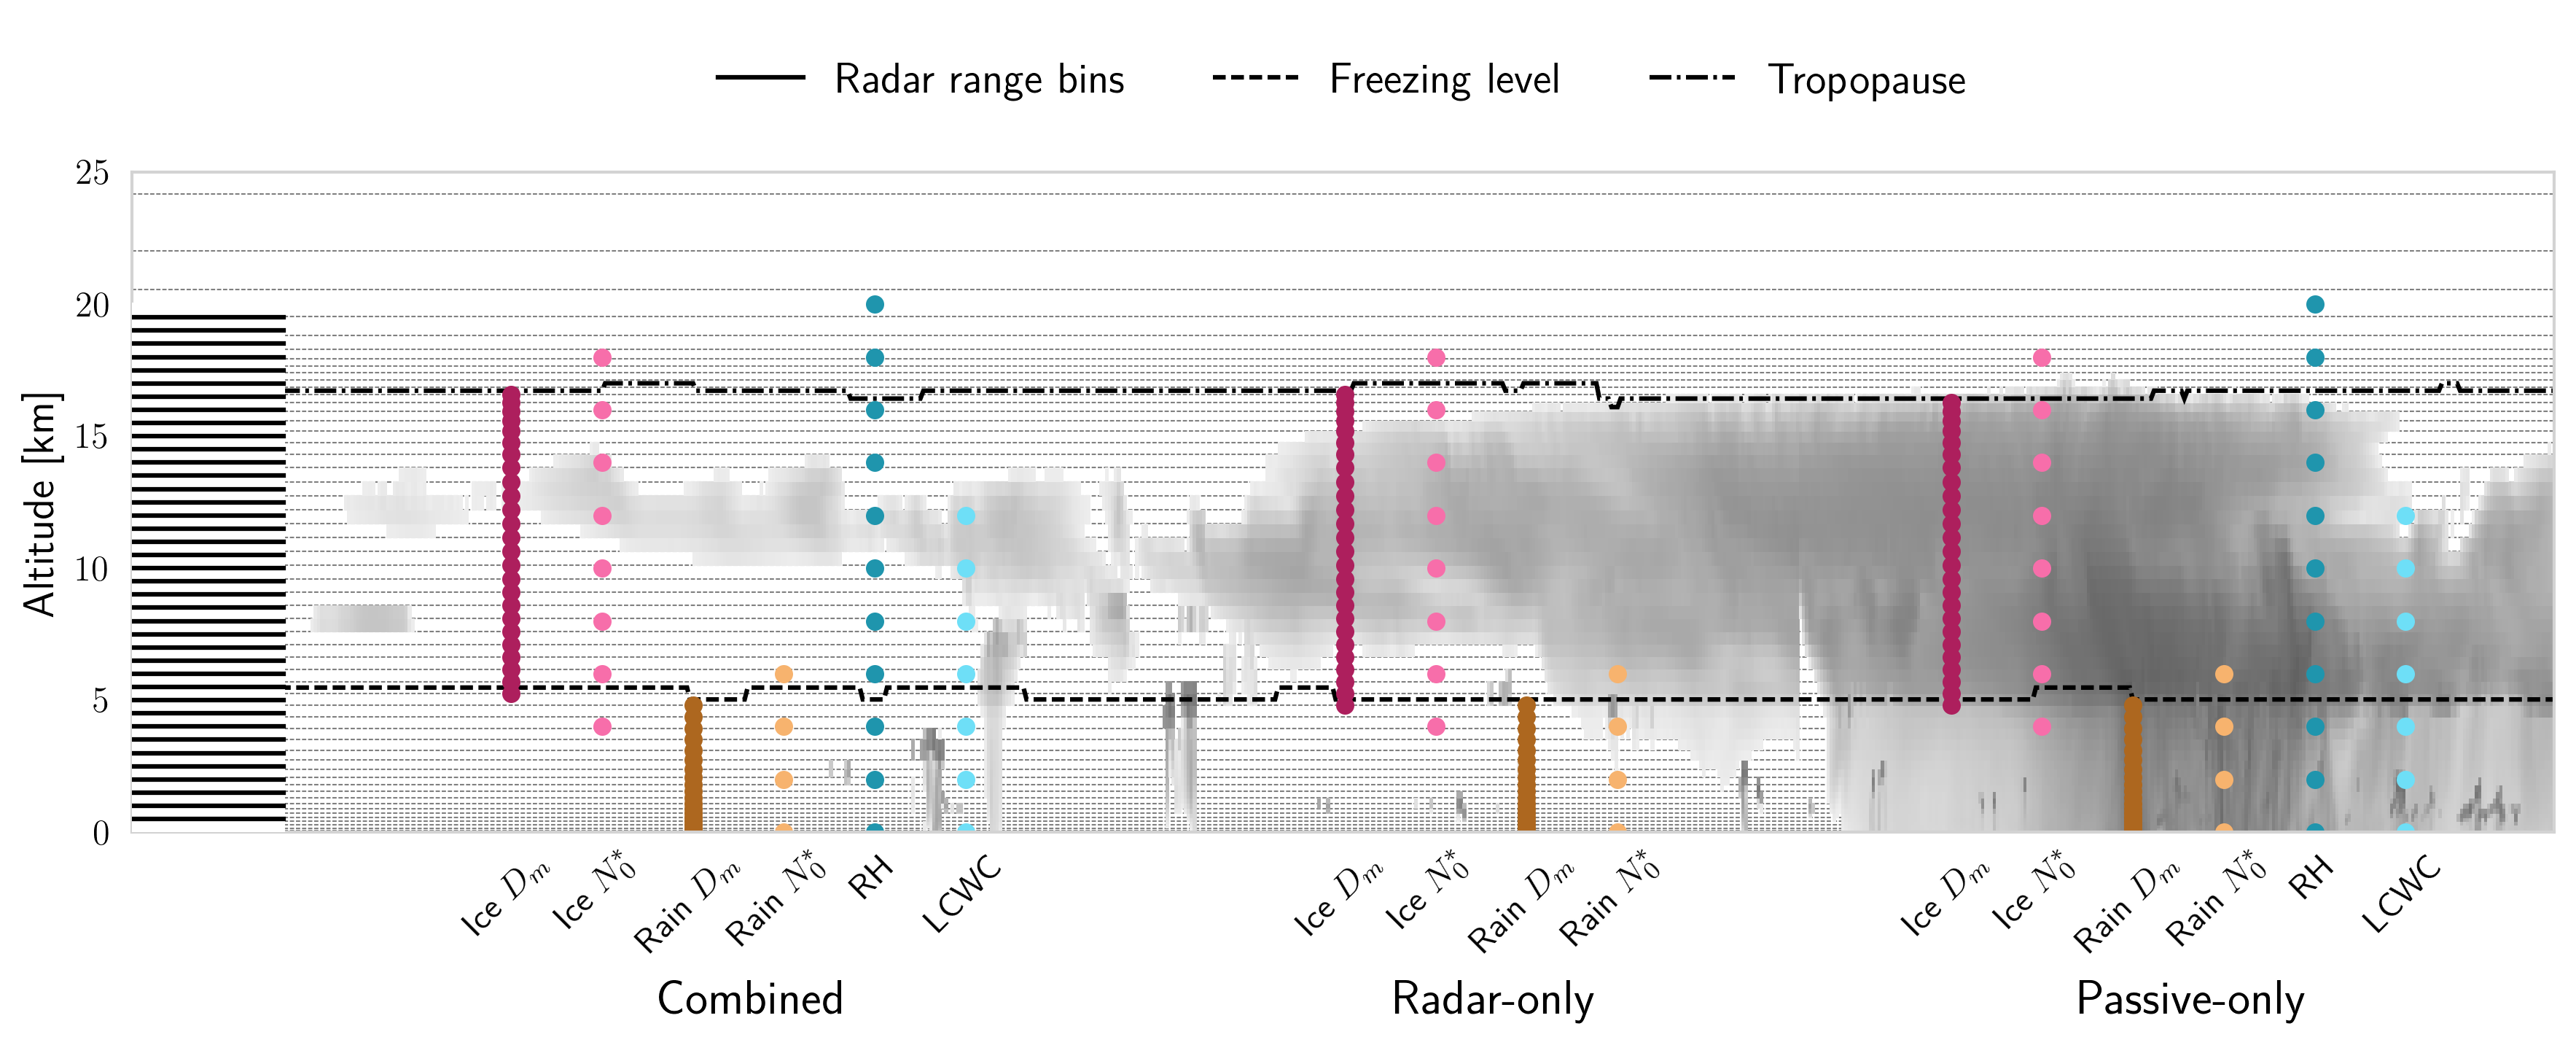
\includegraphics[width = 0.8\linewidth]{../plots/retrieval_sketch}
%\caption{Illustration of the retrieval quantities and their respective retrieval
%  grids. Grey, dashed lines show the resolution of the GEM model data while the
%  filled circles represent the grid points of the different retrieval
%  quantities. Panel (a) shows the configuration used in the radar-only and
%  combined retrieval. Panel (b) shows the configuration used in the passive-only
%  retrieval}
%\label{fig:retrieval_sketch}
%\end{figure}
%
%The motivation for retrieving $N_0^*$ in log-space is that its a priori
%distribution is more similar to a Log-normal rather than a Gaussian distribution
%(see for example \citet{delanoe14}). Since typical values for $D_m$ follow a
%Gaussian distribution rather well these values are retrieved in linear space.
%
%The handling of supercooled liquid in the GEM model scenes is similar to that
%of all other hydrometeors and therefore not explicitly mentioned. In the retrieval,
%liquid cloud is allowed to exist between the surface and the $240\ unit{K}$ isotherm
%and thus also represents supercooled clouds.


\subsection*{Reviewer comment 15}

L 198: Vertical resolution of retrieval grid: Why 4 points? The freezing layer
must be very different for both cased. Maybe a sketch would be helpful as later
on lines 230 the different vertical resolutions for other variables is discussed?

\subsubsection*{Author response}

As mentioned above, the desired sketch will be provided to address this and parts
of the previous comments.

The relatively low number of grid points was found necessary to sufficiently regularize
the retrieval to avoid convergence problems. Except that it was found to work, there is
no exact reason for choosing 4 points. 

The freezing level does indeed vary between the two scenes. The freezing layers of both
scenes will be added to Fig. 1.

\subsection{Reviewer comment 16}

L281: How do I know that Large Plate is the best performing model? Which parameter,plot, table does show that?

\subsubsection*{Author response}

This section will be revised to give more precise recommendation on the choice of the
particle model.
%This sentence is removed in the revised version of the manuscript.

\subsection*{Reviewer comment 17}
L283-L307: Can be shortened significantly

\subsubsection*{Author response}

The proposed change will be adopted in the revised version of the manuscript.

%Following the reviewers recommendations the section will be shortened and
%now  reads as follows:
%
%{\itshape
%Results of the retrieved water content for the first test scene are displayed in
%Fig.~\ref{fig:results_a}. The corresponding results from the second test scene
%are included in Appendix~\ref{app:results_b}. The reference water content is
%defined here as the sum of the masses of the four frozen hydrometeor species in
%the GEM model scenes.
%
%The $\chi^2_y$ value of the different methods, displayed
%in Panel (a), gives an indication of how well the retrievals were able to fit
%the observations. For the radar-only retrieval, the values are far below 1
%for most parts of the scene, while for the passive-only and combined retrieval
%the around 1. This indicates that all methods fitted the observations well over
%the whole scene except for the region around $3^\circ\ N$, where the cloud
%is particularly thick.
%
%In terms of IWP, all methods provide fairly good estimates of the reference IWP
%with the combined retrieval consistently yielding the smallest deviations.
%Larger differences between the methods are observed when comparing the retrieval
%results in terms is IWC. While the vertical structure of the cloud is captured
%only very roughly by the passive retrieval, it much better resolved by the
%radar-only and the combined retrieval. On closer inspection, however, it becomes
%evident that the radar-only retrieval deviates systematically from the reference
%IWC in specific regions of the cloud, such as for example the upper part of the
%cloud between $0^\circ N$ and $2^\circ N$. These deviations are corrected in
%the results from the combined retrieval, although certain retrieval artifacts
%are visible here.}


\subsection*{Reviewer comment 18}
L332: There can I see that? Give figure?

\subsubsection*{Author response}

A reference to the figure will be added in the revised version of the
manuscript.

\subsection*{Reviewer comment 19}
L325: The two paragraph here give similar information -> streamline

\subsubsection*{Author response}

The proposed change will be adopted in the revised version of the manuscript.

%To make the description of the results from the scatter plots more
%concise the section will rewritten as follows:
%
%{\itshape
%Not surprisingly, the results from the
%passive-only retrieval exhibit the strongest deviations from the diagonal. Since
%the passive channels alone contain only limited information on the vertical
%distribution of ice in the atmosphere, the retrieval cannot be expected to yield
%accurate results at the resolution considered here. Although rather weak, a
%certain effect of the ice particle model on the retrieval results can be
%observed. In particular, the GemCloudIce model leads to a systematic
%underestimation of ice mass densities, which are less pronounced for the other
%particle models.
%
%In terms of overall accuracy, i.e. systematic deviations from the diagonal, no
%clear differences between the three configurations are visible. The color-coding
%reveals, however, that the radar-only retrieval is biased for specific
%hydrometeor classes. This effect is less pronounced for the combined retrieval
%and seem to be weaker also in the passive-only results. For Graupel, both the
%radar-only and the combined retrieval perform badly but this due to the radar
%signal saturating in the regions of the scene where Graupel is present (c.f.
%Fig.~\ref{fig:overview} and Fig.~\ref{fig:observations_a}).
%
%Results of all retrievals are affected by the choice of the ice particle model,
%which can cause systematic deviations especially at high IWC values. For the
%radar-only results these deviations are smallest for the LargeColumnAggregate,
%whereas for the combined retrieval the LargePlateAggregate and 8-ColumnAggregate
%yield the most accurate results.}


\subsection*{Reviewer comment 20}
L333-344: I would put this to the appendix

\subsubsection*{Author response}

We will follow the reviewers advice and put the analysis of the second test scene
into the appendix.

\subsection*{Reviewer comment 21}
L444: Here it needs to be made clearer how this goes beyond what GPM is doing.


\subsubsection*{Author response}

To clarify how our work goes beyond what GPM a paragraph detailing this
will be added to the discussion.

%To clarify how our work goes beyond what GPM is doing the following paragraph
%will be added to the manuscript:
%
%{\itshape The novelty of this work lies, for one part, in the application of ICI's
%sub-millimeter channels, which sets it apart from the combined retrievals
%developed for the TRMM and GPM missions. For the other part, it lies in the
%development of a fully-consistent variational retrieval in which all retrieval
%quantities are retrieved from the observations from all sensors simultaneously.
%This allows comparing the retrieval to equivalent radar-only and passive-only
%configurations and therefore a direct analysis of the synergies between the
%active and passive observations.}

\subsection*{Reviewer comment 22}
L495:  “does not say much about the general validity of the assumption”.   Here you should dig in a bit more. What is the role of a priori and covariances?

\subsubsection*{Author response}

Following the suggestion of the reviewer we will extend the discussion
of the a priori assumptions.

%To extend the discussion of the role of the a priori assumptions in the retrieval
%the corresponding paragraph will be modified as follows:
%
%{\itshape 
%  The a priori assumptions which were used in this study were similar but not
%  identical to what is used in the DARDAR retrievals. Also here it should be
%  noted, that the presented results should not be taken to be representative for
%  the DARDAR product. Rather than this, the DARDAR a priori settings were chosen
%  since they represent well established and validated assumptions for ice cloud
%  retrievals and therefore should provide a reasonable starting point for the
%  development of a combined cloud retrieval. Although the a priori assumptions
%  work well for the first test scene they lead to systematic error in the second
%  scene. The analysis in Fig.~\ref{fig:results_scatter} shows that the cause for
%  this is the composition of the cloud. The a priori works well if the scene
%  contains both snow and ice but causes systematic errors when this is not the
%  case. The role of the a priori is to complement the observations with additional
%  information in order to make the retrieval problem tractable. For the radar-only
%  retrieval this means that the a priori determines how the information from a
%  single range gate is distributed between the two degrees of freedom of the
%  particle size distribution. Since the degrees of freedom vary more or less
%  independently from each other, no a priori can fit for every possible cloud
%  configuration.
%}

\subsection*{Reviewer comment 23}
L560:  Rethink the bullet structure.  2.  Is not an independent result.  For each resultrefer to the part of the manuscript where you can clearly see that.  Especially result 3 should be detailed – how do ICI channel advance the currently available data?

\subsubsection*{Author response}

The bullet points will be remove in the revised manuscript and replaced
by text.

%To improve the presentation of the conclusions, the bullet points will be removed
%and the first paragraphs of the conclusions will be rewritten as follows:
%
%{\itshape The main conclusion from this work is that the combination of radar and
%  sub-millimeter radiometer observations allows to constrain both the size
%  as well as the concentration of frozen hydrometeors. The sensitivity of
%  the combined observations to the microphysics of the cloud reduced the
%  median bias in the retrieved IWC from more than $50\ \%$ in the radar-only
%  to less than $10\ \%$ for suitable choices of the particle model (Fig.~\ref{fig:boxes}).
%
%  Our results particularly highlight the importance of sub-millimeter observations
%  for combined retrievals of frozen hydrometeors. While observations at currently
%  available microwave frequencies provide only limited complementary information
%  to the radar observations, it is mainly the frequencies above $200\ \unit{GHz}$
%  that provide additional information on cloud microphysics (Fig.~\ref{contours})
%  for
%
%  Moreover it has been found that the combination of radar and passive microwave
%  observations may help the retrieval of mixed-phase clouds. Since the role of
%  these clouds in the climate of the arctic are an active topic of study, the use
%  of combined sub-mm/radar observations should be further investigated.}


\subsection*{Reviewer comment 24}

Fig.  3: Is it really worth having the slightly different size distribution shapes for frozen and liquid? Isn’t there a stronger difference between different frozen hydrometeors

\subsubsection*{Author response}

This is certainly true but in most clouds ice and rain can be distinguished a
priori, which simplifies using different PSD shapes for the liquid and frozen
hydrometeors. Distinguishing between different frozen hydrometeors is difficult
to do a priori and using multiple species of hydrometeors in the retrieval was
found to cause ambiguities that the retrieval is not able to resolve.


%We agree with the reviewer that the slightly different size distributions shapes likely do
%not affect the retrieval significantly. The choice of the PSD parameters for liquid
%hydrometeors was made rather arbitrarily, but since the retrieval was found to work
%the effect of the PSD parameters has not been investigated further.

\subsection*{Reviewer comment 25}
Figures 7 and 8:  I’m not sure why these are separate figures – it seems like allpanels could fit on one page.

\subsubsection*{Author response}

Figures 7 and 8 will be combined into a single figure in the revised manuscript.

\subsection*{Reviewer comment 26}
Fig. 4 and also in text: “cloud signal” say that this is dTB.

\subsubsection*{Author response}

Following the reviewers recommendation, the passive cloud signal will be
referred to in the text as $\Delta T_B$ and the radar signal as
$\text{dBZ}_\text{max}$.

%The corresponding paragraph will also be changed
%to make it more concise:
%
%{\itshape 
%The question that is addressed here is whether the combination of active and
%passive observations is able to constrain both the size and concentration of the
%ice particles in the cloud. To investigate this, the $N_0^*$ and $D_m$
%parameters of the homogeneous cloud layer are varied and observations of the
%cloud layer are simulated. The passive cloud signal ($\Delta T_B$) is the
%difference between the cloudy- and clear-sky  brightness temperatures. The
%signal in the active observations is here defined as the maximum in the measured
%profile of radar reflectivity $\text{dBZ}_\text{max}$. Figure~\ref{fig:contours}
%displays the contours of $\Delta T_B$ and $\text{dBZ}_\text{max}$ with respect
%to $D_m$ and the clouds IWC, which is proportional to $N_0^*$:
%\begin{align}
%m = \frac{\pi \rho}{4 ^ 4}N_0^* D_m^4,
%\end{align}
%where, $\rho$ is the density of ice.
%
%  }
%
%
%The proposed change will be adopted in the updated version of the manuscript.

\subsection*{Reviewer comment 27}
Fig. 5: Can you add freezing layer height?

\subsubsection*{Author response}

We propose to add the freezing layer height to Fig.~1 as it will then
also show the freezing layer height for the second scene and with
this address minor comment 15.

%Freezing layer has been added to Fig.~5, which now looks as follows:
%
%\begin{figure}
%\centering
%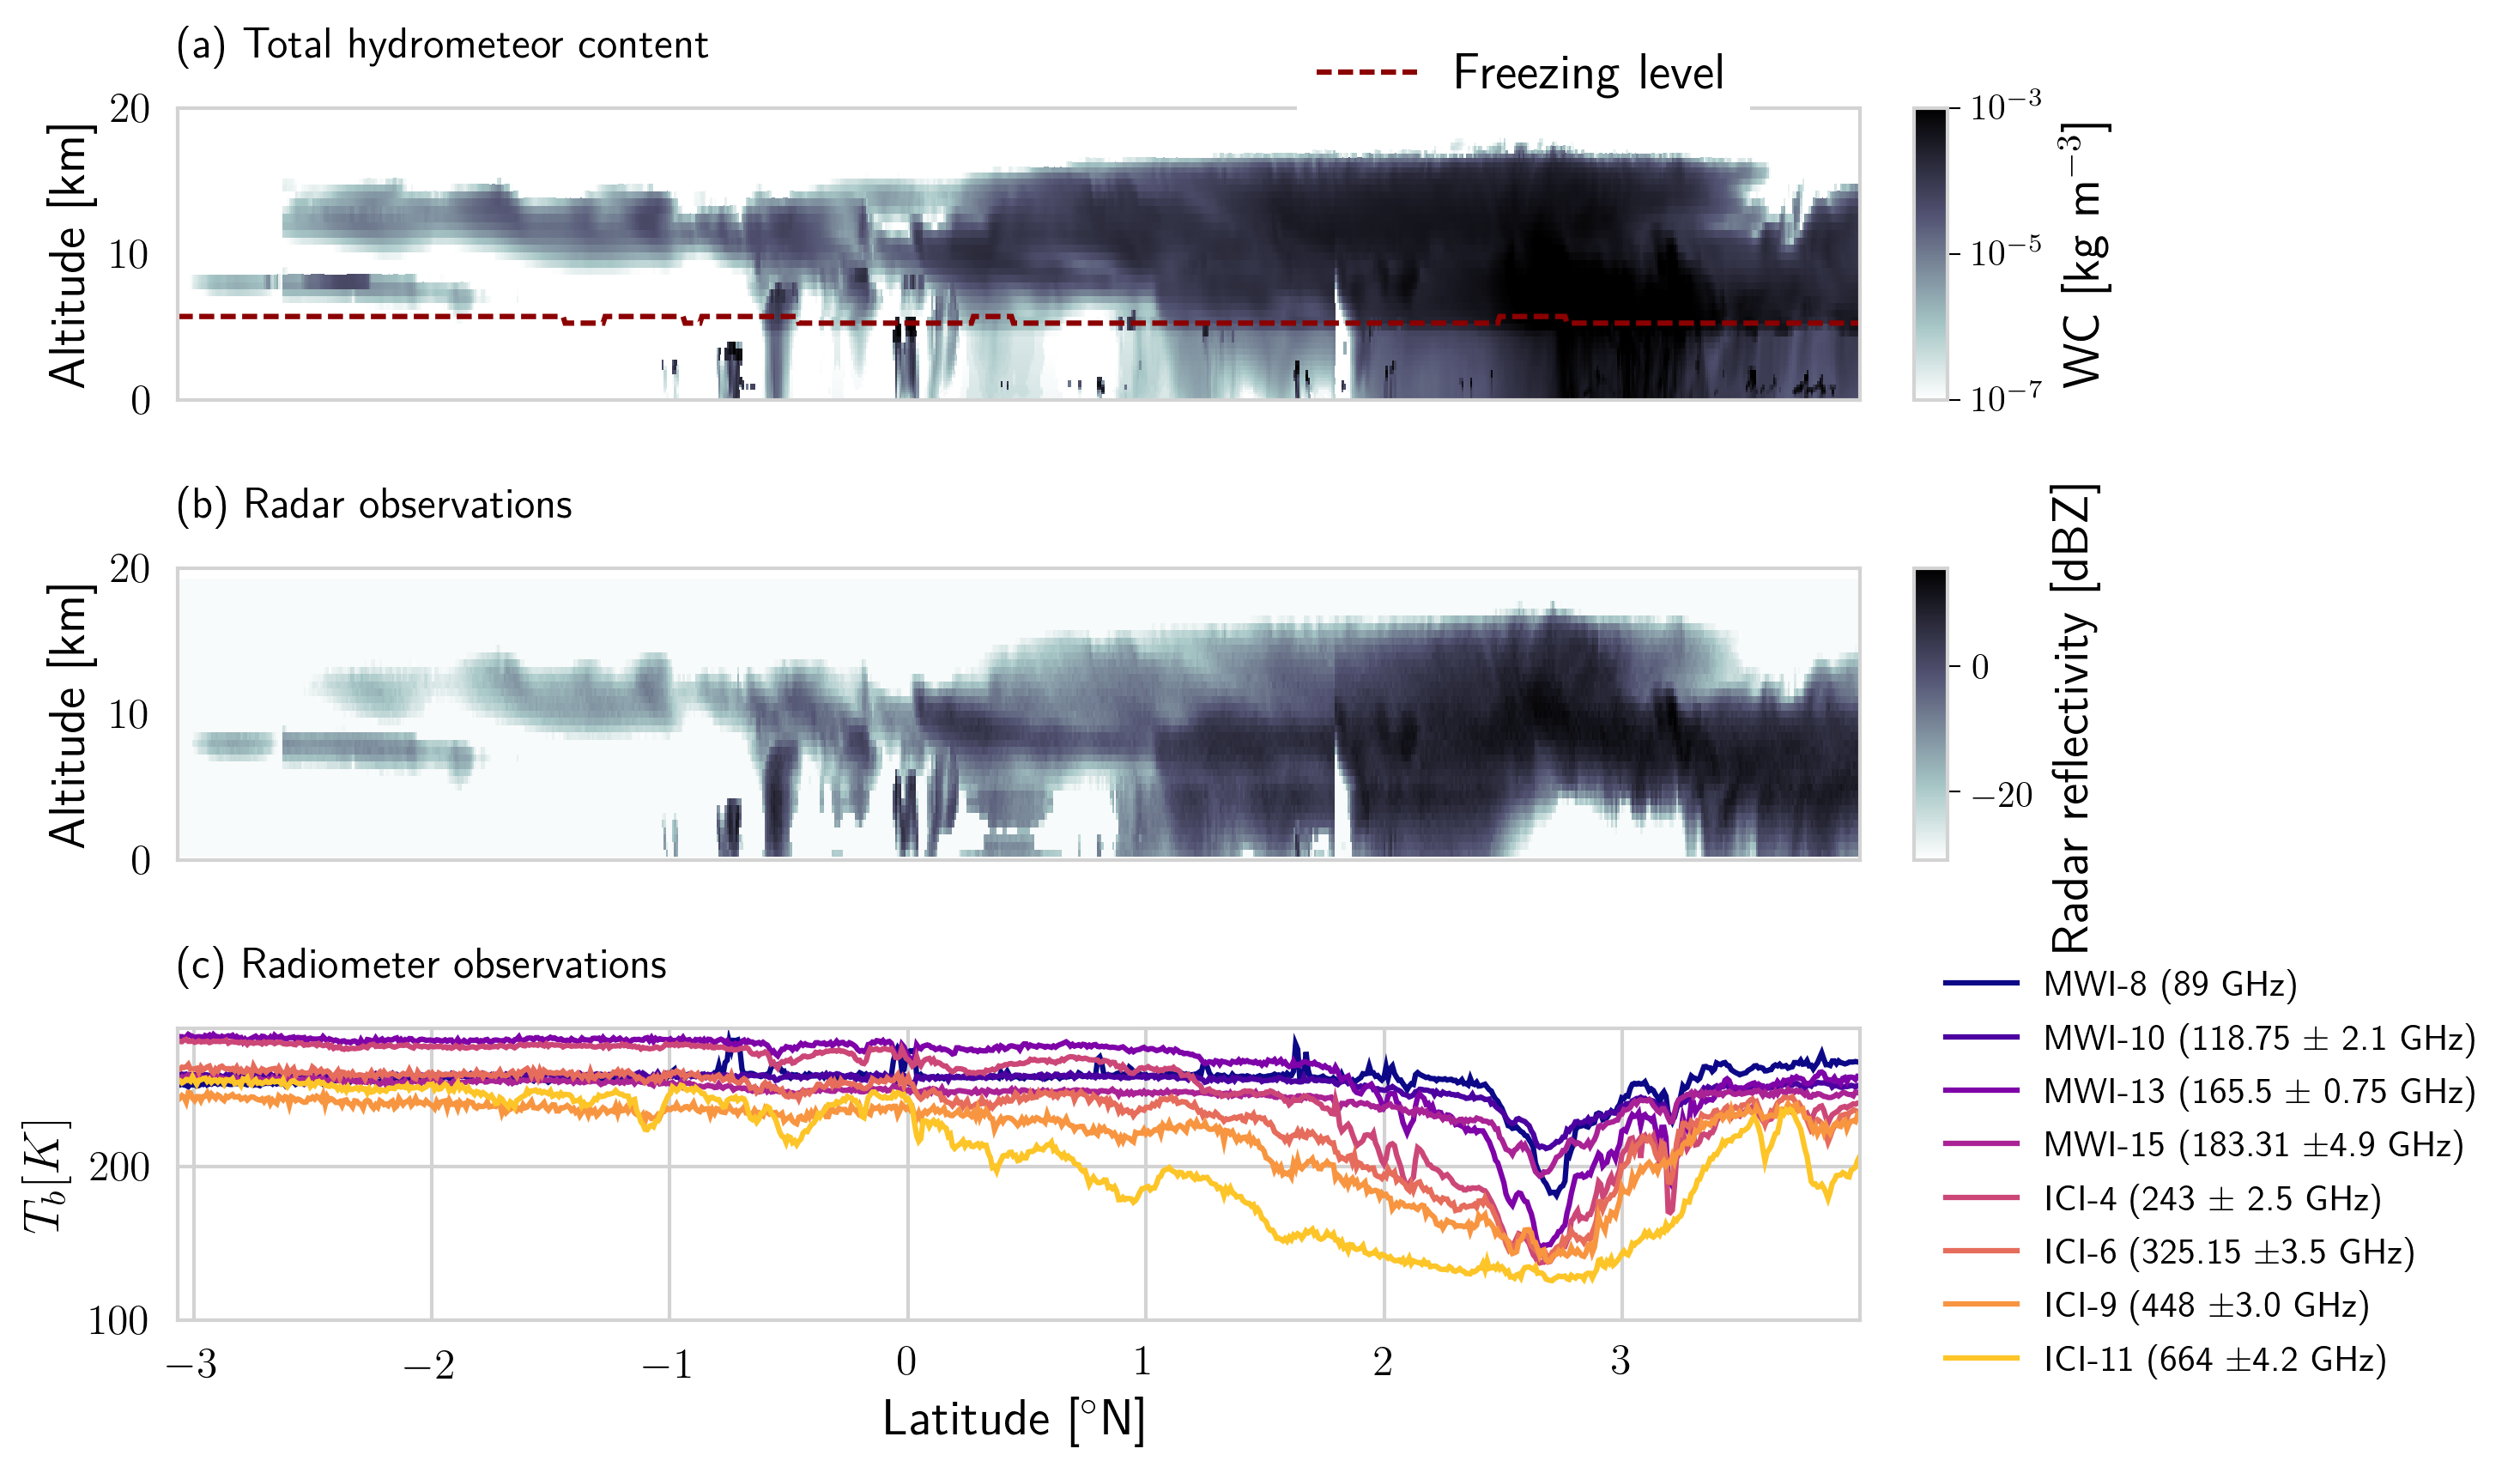
\includegraphics[width = 0.8\textwidth]{../plots/observations_a.png}
%\caption{Total hydrometeor content (HMC) and simulated observations for the first test
%  scene. Panel (a) displays the total hydrometeor content in the scene, i.e. the
%  sum of the mass densities of all hydrometeor species of the GEM model. Panel
%  (b) shows the simulated radar reflectivities. Panel (c) displays the simulated
%  brightness temperatures for a selection of the channels of the MWI and ICI
%  radiometers.}
%\label{fig:observations_a}
%\end{figure}


\subsection*{Reviewer comment 28}
Fig.  6:  It would be nice to see the absolute values of IWP somewhere.  Maybe youcould add another time series with IWP as the sum of the different components such that the reader can see where the different categories (cloud, graupel, snow and hail) contribute most?

\subsubsection*{Author response}

To address the reviewers request we will the absolute reference IWP and its
decomposition into different hydrometeor classes to Fig. 6.

%To address the reviewers request the figure will be modified as follows:
%
%\begin{figure}
%\centering
%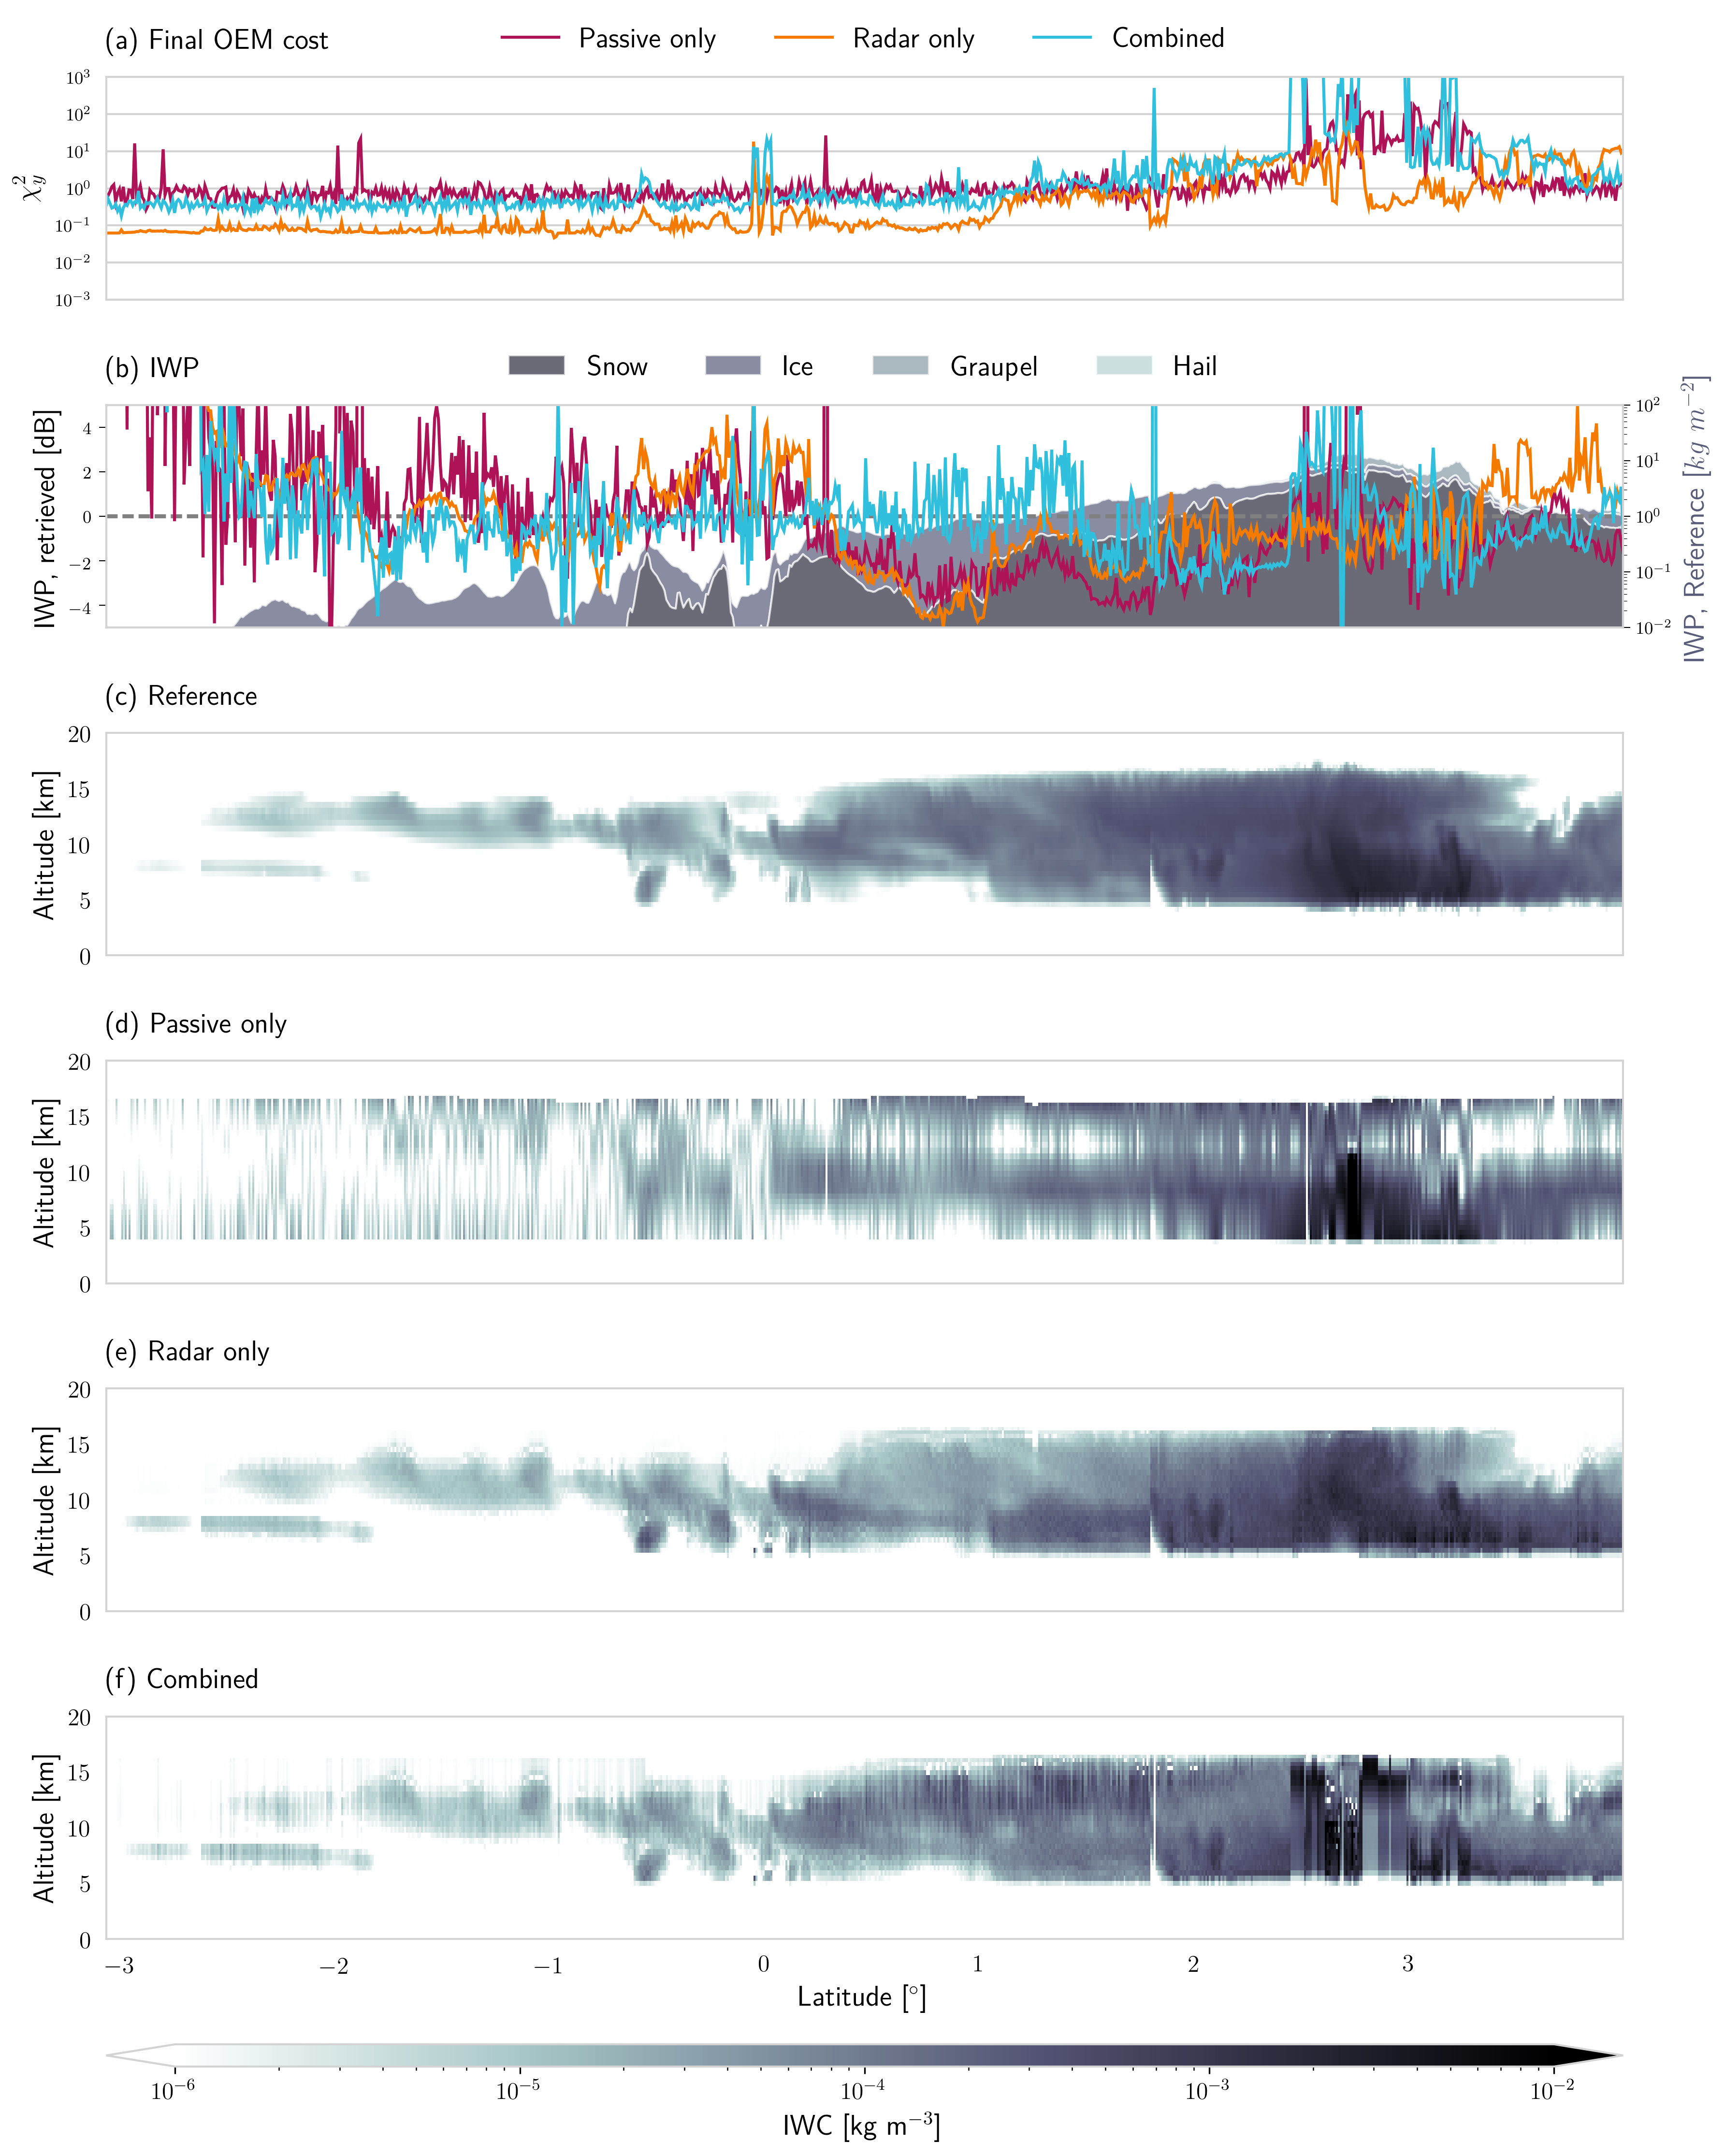
\includegraphics[width = 0.8\textwidth]{../plots/results_a_LargePlateAggregate.png}
%\caption{Results of the ice hydrometeor retrieval for the first test scene.
%  Panel (a) displays the value of the $\chi^2_y$ diagnostic normalized by the
%  dimension of the measurement space of the corresponding retrieval. Panel (b)
%  displays retrieved IWP in dB relative to the reference IWP. Panel (c) shows
%  the reference IWC from the model scene. Panel (d), (e) and (f) display the
%  retrieval results for the passive-only, radar-only and combined retrieval,
%  respectively.}
%\label{fig:results_a}
%\end{figure}


\subsection*{Reviewer comment 29}
Fig.  7:  I think it is retrieved vs.  truth.  The word following is not really exact.  Why not put 7 and 8 together?

\subsubsection*{Author response}

Fig. 7 and 8 will be merged and the label will be corrected.

%The following will be corrected and Fig. 7 and 8 will be combined into 1 to look as follows:
%
%\begin{figure}
%\centering 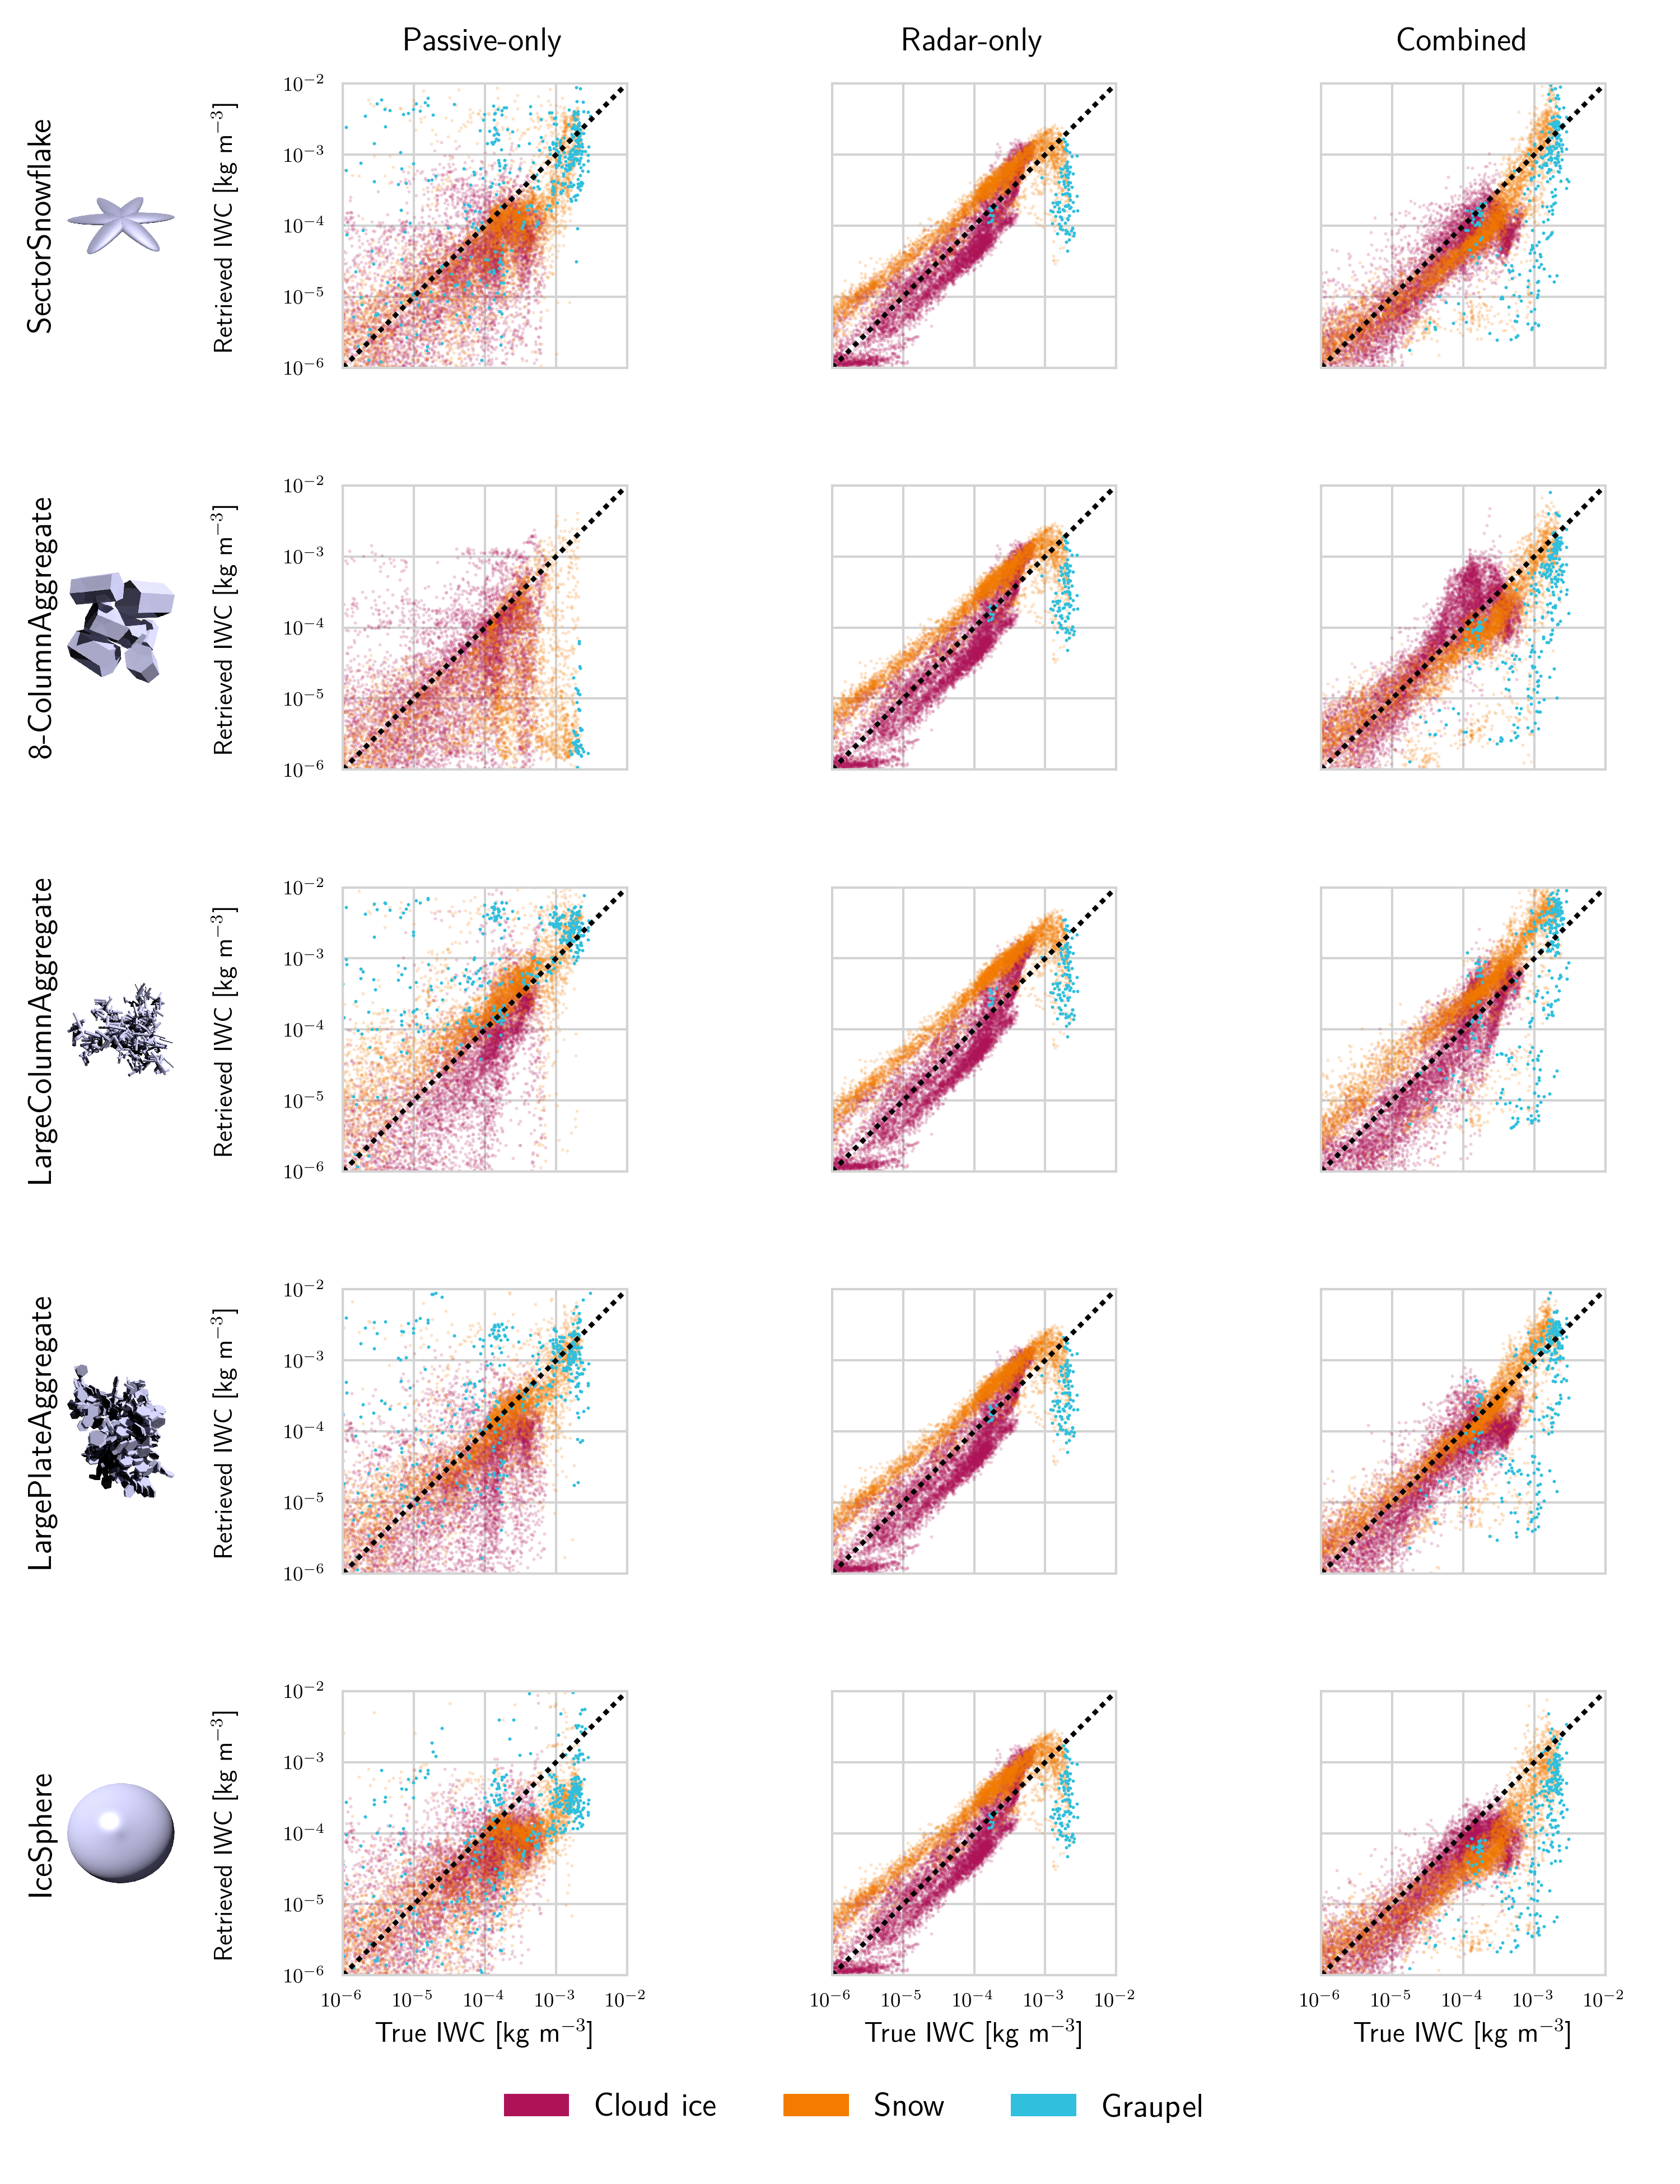
\includegraphics[width = 0.8\textwidth]{../plots/results_scatter_a.png}
%\caption{Retrieved IWC plotted against reference IWC for the tested retrieval
%  configurations. Each row shows the retrieval results for the particle shape
%  shown in the first panel. The following panels show the retrieval results for
%  the passive only (first column), the radar only (second column) and the
%  combined retrieval (third column). Markers are colored according to the
%  prevailing hydrometeor type at the corresponding grid point in the test
%  scene. Due to their sparsity, markers corresponding to graupel are drawn at
%  twice the size of the other markers.}
%\label{fig:results_scatter_a_1}
%\end{figure}

\subsection*{Reviewer comment 30}
Fig. 9: Could go to the appendix

\subsubsection{Author response}
Fig.~9 will be moved to the appendix.

\subsection*{Reviewer comment 31}
Fig. 10 I only see the caption???

\subsubsection*{Author response}

Fig. 10 was unfortunately missing from the manuscript. The figure will be included in the appendix
with the analysis of the second test scene.

\subsection*{Reviewer comment 32}

Tab. 1. Assumed particle model information for each hydrometeor class given by GEMmodel. In fact it could be good to combine it

\subsubsection*{Author response}

Tables 1 and 4 will be combined in the revised version of the manuscript.


\section*{Grammar, typos and reformulations}

The authors would like to thank the reviewer for the additional comments which all
will be incorporated into the revised manuscript.


\bibliographystyle{copernicus}
\bibliography{references}

\end{document}
